\chapter{Problems Identified in UD Treebanks}
\label{sec:problems}

Ever since the UD project was introduced in 2014, and since the revision of guidelines in UDv2, there have been multiple publications that highlight the problems in UD treebanks. Some of the problems highlighted in these publications have been found to be global in nature (i.e. they occur in almost all treebanks, regardless of the language), while the others are related to a specific group of languages. Before we start discussing the problems, we shall specify the general kind of errors.

\cite{error-types} define different kinds of errors that can be found in a treebank. The first kind are the random errors, characterised by the inconsistencies introduced by the annotators owing to the distractions while undertaking the annotation procedure. The systematic and recurrent errors are introduced not in isolated scenarios as random errors, but can be found across the treebank in a consistent manner. These errors are usually related to the guidelines of the treebank, in either of two ways. The guidelines could be misunderstood by the annotator(s), and/or the guidelines might themselves be unclear (or not appropriate to handle some cases), leaving the annotator(s) in a jeopardy. \cite{alzetta2017dangerous} extend the definition of systemic and recurrent errors to also include the cases of conversion errors, caused by improper mapping of original annotation scheme to a new scheme. Throughout the length of this document, we focus on the errors of the second kind (systemic and recurrent errors), and try to correct them.

It is worth pointing out why the experiments listed in the section were chosen to work on, and not others. As we will see, apart from the first problem listed in next few sections, almost all of the error typologies were pointed out from a common source \citep{alzetta2017dangerous}. The authors of the paper note that the mined patterns were found to be common across different sections of the \verb|it| treebank, and across different languages as well. Owing to the success of the algorithm in determining the typology of inconsistencies, it makes sense to use it on different datasets to flag (and correct) the inconsistencies within them as well.

\section{Annotation Consistency in Different Treebanks}
\label{sec:harmony}

UDv2.5 \citep{UDv2.5}, as mentioned earlier, contains 157 treebanks in 90 languages. As such, there are multiple languages with more than one treebank, with some containing up to 6 treebanks. A list of languages in UDv2.5 such that they contain more than one treebank is listed in Appendix \ref{app:multi_trees}. Regardless of the differences in genre or the teams involved for building the treebank, the different treebanks for a language should be consistent with respect to the annotation guideline(s), both intra and inter treebanks. However, this is often not the case, primarily because of the different sources of origin of the individual treebanks.

The problem of determining the degree to which the different treebanks differ from each other has been studied in some detail over multiple years, but is not yet entirely solved. We discuss the different solutions proposed over time regarding this problem in Sections \ref{ssec:inconsistency-detection-pos} and \ref{ssec:inconsistency-detection-deprel}.

We return to this problem in Chapter \ref{chap:pos-harmony}, when we try to devise a metric to compare the different treebanks on basis of their POS annotation.

\section{Problems Caused by Change of Guidelines in UDv2}
\label{ssec:guidelines}

A summarized version of changed guidelines from UDv1.x to UDv2 can be accessed online\footnote{\url{https://universaldependencies.org/v2/summary.html}}. Most of the changes in guidelines could be processed in an automatic manner. For example the renaming of particular POS tags or dependency relations could be implemented across the different treebanks in a deterministic manner. However, there were some changes that could not be applied deterministically, and those form the majority of the problems in this section.

It is important to note that the changes had to be applied to 64 treebanks in 47 languages as they moved from UDv1.4 to UDv2.0, and so the analysis might be limited to these 64 treebanks only in this case. However, it is worth scouting for these patterns in the newer treebanks, given how some (if not all) of them might be a cause of concern therein.

The task of POS tagging, and dependency parsing of the input sentences were done with the help of UDPipe \citep{UDPIPE}, which contains the trained models for UDv1.2, UDv2.0, UDv2.3 and UDv2.4. The dependency tree structures shown throughout the length of this document are generated as per Parsito format \citep{Parsito}.

\subsection{Conversion Errors in Conjunctions}
\label{sssec:conj_head}

In the changed guidelines, there were two changes with respect to conjunction tags \verb|CCONJ| and \verb|SCONJ|; and the dependency relations, \verb|cc| and \verb|conj|. The changes are listed as follows:

\begin{enumerate}
    \item The POS tag \verb|CONJ| in UDv1 was changed to \verb|CCONJ| in UDv2, to make it more parallel to \verb|SCONJ|.
    \item The conjunctions are attached to the immediately succeeding conjunct in UDv2, as opposed to UDv1 where they were attached to the first conjunct.
\end{enumerate}

Of the two changes in guidelines, the first one (renaming of tag) can be applied deterministically, and automatically throughout the treebank(s). The second change, however, can be classified as head identification error. The pattern in question (referred to as \texttt{conj\_head} henceforth) was also identified by \cite{alzetta2017dangerous} in their paper, where they note that it contributes to 24.65 \% of total discovered error instances. This implies that this is indeed a major error category, and needs to be handled well. We do take a look at this error type in Chapter \ref{chap:conj_head} where we discuss about it in detail.

\subsection{\texttt{AUX} and \texttt{VERB} Distinctions}
\label{ssec:AuxVERB}

The following is a list of changes for the category of auxiliaries from UDv1.4 to UDv2:

\begin{enumerate}
    \item The definition of \verb|AUX| was extended to include copula verbs, and non-verbal TAME (Time, Aspect, Mood, Evidentiality. Might/might not include Voice and Polarity) particles.
    \item The \verb|aux| relation was also expanded to include non-verbal TAME particles, as in the case of \verb|AUX|.
    \item The relation \verb|auxpass| was removed from UDv2.0, making it as a subcategory of the larger \verb|aux| relation, in the form of \verb|aux:pass|. Essentially speaking, \verb|auxpass| was demoted to a sub-category of \verb|aux| relation.
\end{enumerate}

Considering the changes that the auxiliaries went under with the change in guidelines, the line of distinction between the POS \verb|VERB| and \verb|AUX| became fuzzier. At the time of writing this document, the distinction between the two is not always explicit. For a given language, this is also governed by the definition of the terms in UD, and how those definitions agree with the traditional language-grammar. This is noted in part in the guidelines for UDv2 as well, where the following point is noted, with reference to the definition\footnote{\url{https://universaldependencies.org/u/pos/all.html\#aux-auxiliary}} of \verb|AUX|:

\begin{verbatim}
[AUX] is often a verb (which may have non-auxiliary uses as 
well) but many languages have nonverbal TAME markers and
these should also be tagged AUX.
\end{verbatim}

One of the proposed change in guidelines was to get rid of \verb|AUX| altogether\footnote{\url{https://github.com/UniversalDependencies/docs/issues/275}}. However, as per findings of \cite{de2016should}, a parser is not able to learn the distinction between the two categories, when they are merged together. The authors observe a decrease in parsing scores when the two categories are not explicitly separated. This was the principal motivation behind keeping the two separate. However, there still exist problems with respect to the differentiation between the two categories, as can be seen in the list of open issues on the subject\footnote{\url{https://github.com/universaldependencies/docs/issues?utf8=\%E2\%9C\%93&q=is\%3Aopen+aux}}.

In UDv2.4, it was proposed to limit the \verb|AUX| by a list. The list would essentially identify all auxiliaries by a common definition, and thus would be able to create a better distinction between the two conflicting categories of \verb|AUX| and \verb|VERB|. This could be realized just in part though, principally because of the conflicts between traditional grammar-based definitions of the two categories, and the definitions as per UD.

With respect to this particular error type, we tried to segregate the classes of \verb|AUX| and \verb|VERB| in our experiments in Chapter \ref{chap:failures}, without using the aforementioned list. 

\section{Non-projective Structures}
\label{ssec:nonproj}

While non-projectivity is not tackled as an issue in the scope of the current research, it is nonetheless an important linguistic phenomenon that warrants attention. In this section, we cover the concept as a primer, such that the reader is not lost about the topic when it is referred to in future chapters. We discuss an open problem about non-projective structures later in Section \ref{future:nonproj}. 

Let us understand non-projectivity through the following example from LinES treebank in \verb|en| data, and the tree structure as shown in Figure \ref{fig:nonprojdemo}.

\begin{figure}[h]
    \centering
    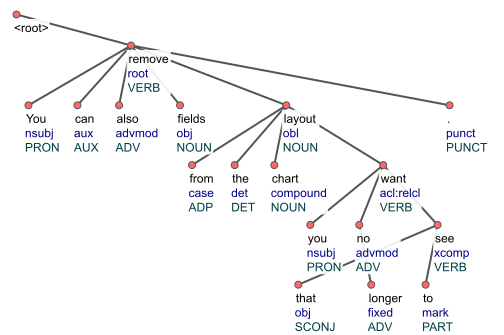
\includegraphics[scale=0.75]{img/nonproj-demo}
    \caption{Sample Non-projective Tree}
    Note: \textit{that} should be tagged as \texttt{PRON}, and not as \texttt{SCONJ}
    \label{fig:nonprojdemo}
\end{figure}

In the graph, notice the edge going from \textit{see} to \textit{that}. We can see that the edge crosses over another edge in order to link the two tokens. Informally, presence of such crossing edges in a tree makes it non-projective in nature.

\subsection{Related Terms and Formal Definition}

To define the concept of non-projective structures in a formal manner, we need to define a few notations. We use the same notations as used by \cite{mambriniNonProj}.

If a node \(j\) depends on a node \(i\), we call node \(j\) as a child node of \(i\) (also, \(i\) is parent node of \(j\)), represented as \(i \xrightarrow{} j\). We use \(i < j\) to denote the node \(i\) preceding node \(j\) in the tree \(T\). A node \(v\) lying in between the nodes \(i\) and \(j\) in the tree can be represented as \(v \in (i,j)\). Also, we use the notation \(v \in Subtree_{i}\) if node \(v\) is part of the subtree rooted at node \(i\). 

From \cite{Havelka}, we can define the condition of projectivity of a tree as follows:

\theoremstyle{definition}
\begin{definition}
\label{def:projectivity}
A given tree \(T\) is projective in nature iff
\begin{equation}
\label{eqn:projectivity}
    i \xrightarrow{} j \And v \in (i, j) \implies v \in Subtree_{i} \qquad \forall i, j, v \in T 
\end{equation}

If a given tree does not satisfy the above condition, it is said to be non-projective in nature. Furthermore, in case of non-projectivity, node \(v\) is said to be in gap, represented as \(v \in Gap_{i\leftrightarrow}j\). The double headed arrow signifies the nodes being considered irrelevant of their order of occurrence in the tree.
\end{definition}

\cite{mambriniNonProj}, in their work on \verb|grc|, highlight that the distribution of non-projective structures might be affected by genre distribution. In particular, poetic style is liable to contain more non-projective structures than prose. The claim about genre distribution affecting projectivity is also supported by \cite{nonprojgenre}, where they look at different genres (news and conversations) using different parameters to account for lack of non-projective structures in the conversational genre, than in news genre. %Although more research is needed on the topic, we try to base our experiments while restricting ourselves to the genre distributions that are more or less alike (cf. Section \ref{sec:nonproj_dataset} and discussion of \texttt{support treebanks}).

\subsection{Punctuation Induced Non-Projectivity}
\label{ssec:punct-nonproj}

A punctuation node can induce non-projectivity in either of the two ways as mentioned below:

\begin{enumerate}
    \item Non-projective attachment of a punctuation node.
    \item Non-projectivity caused by only punctuation node(s) in gap.
\end{enumerate}

According to UD guidelines, a punctuation node should be attached to the surrounding dependent unit. However, it is not always possible to identify the correct dependent where the node should be attached. Consider the following example from \verb|en|-lines UD v2.5 treebank, and the associated dependency tree in Figure \ref{fig:punct-nonproj}, with specific reference to the punctuation mark immediately following the token marked in bold. While the punctuation token could have been correctly marked to either of \textit{right} or \textit{said}, it is attached to \textit{'s} causing non-projectivity.

\begin{example}
That's \textbf{right}, said Quinn.
\end{example}

\begin{figure}[H]
    \centering
    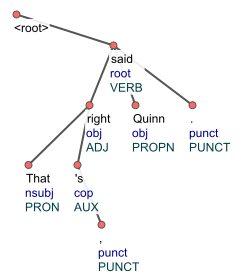
\includegraphics{img/punct-nonproj.png}
    \caption{Punctuation Node Attached Non-Projectively}
    \label{fig:punct-nonproj}
\end{figure}

Similarly, the punctuation node(s) can induce non-projectivity, by attaching itself to the wrong node. Consider the following example from \verb|en|-EWT UDv2.5 treebank, and the associated dependency tree in Figure \ref{fig:punct-nonproj2}, with specific reference to the punctuation mark immediately following the token in bold. A faulty association of this punctuation induces non-projectivity in another node.

\begin{example}
Analyst Team 1 : \textbf{Coach} : Lisa Gilette
\end{example}

\begin{figure}[H]
    \centering
    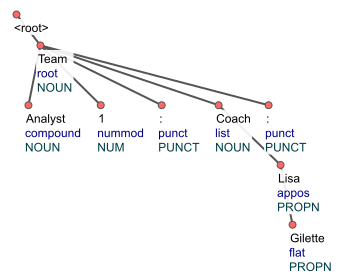
\includegraphics{img/punct-nonproj2.png}
    \caption{Punctuation Node Causing Non-Projectivity}
    \label{fig:punct-nonproj2}
\end{figure}

To summarise, we can say that a non-projective edge \(i \rightarrow j\) is a case of Punctuation Induced Non-Projectivty if any of the following conditions are met:

\begin{enumerate}
    \item Either of head (node \(i\)), or dependent (node \(j\)) is a punctuation node.
    \item The nodes in \(Gap(i, j)\) consist of \textbf{only} punctuation node(s).
\end{enumerate}

Projectivity in itself is a strict constraint for a multitude of natural languages. Therefore, there have been multiple relaxations that have been suggested over time on the strict constraint of projectivity. Appendix \ref{app:nonproj-relaxations} discusses some of these relaxations, and then lists in tabular form the statistics related to non-projectivity in different treebanks in UDv2.5 data.